%%%% dcml.tex

\typeout{IJCAI-09 Instructions for Authors}

% These are the instructions for authors for IJCAI-09.
% They are the same as the ones for IJCAI-07 with superficical wording
%   changes only.

\documentclass{article}
% The file dcml.sty is the style file, copied from the style file for IJCAI-09 (same as ijcai07.sty).
\usepackage{dcml}

% Use the postscript times font!
\usepackage{times}

% For tables:
\setlength{\tabcolsep}{0.25\tabcolsep}
\usepackage{float}

\usepackage{graphicx}
\graphicspath{ {img/} }


% the following package is optional:
%\usepackage{latexsym} 

% Following comment is from ijcai97-submit.tex:
% The preparation of these files was supported by Schlumberger Palo Alto
% Research, AT\&T Bell Laboratories, and Morgan Kaufmann Publishers.
% Shirley Jowell, of Morgan Kaufmann Publishers, and Peter F.
% Patel-Schneider, of AT\&T Bell Laboratories collaborated on their
% preparation.

% These instructions can be modified and used in other conferences as long
% as credit to the authors and supporting agencies is retained, this notice
% is not changed, and further modification or reuse is not restricted.
% Neither Shirley Jowell nor Peter F. Patel-Schneider can be listed as
% contacts for providing assistance without their prior permission.

% To use for other conferences, change references to files and the
% conference appropriate and use other authors, contacts, publishers, and
% organizations.
% Also change the deadline and address for returning papers and the length and
% page charge instructions.
% Put where the files are available in the appropriate places.

\title{Predicting clinical features based on RNA-protein correlations in cancer patients}
\author{Hannah Boekweg, Corbin Day, Caleb Lindgren \\
Department of Biology\\
Brigham Young University}

\begin{document}

\maketitle

\begin{abstract}
  Cancer patients have abnormal RNA/protein correlations, compared to healthy patients.
  We use various metric of aberrant RNA/protein correlations as features to predict clinical features (e.g survival) of cancer patients.
  We assess the accuracy achieved by three different models: MLP, KNN, and Naive Bayes. For survival and recurrence, all models achieve the ~80 percent accuracy. For other features Naive Bayes outperformed MLP and KNN.

\end{abstract}

\section{Introduction}
There are several molecular process that occur in order for proteins, which perform the function of cells, to be made. 
It begins with DNA (the instructions for the cell), which gets transcribed to RNA (the messenger), which is then able to be translated to proteins. 
Proteins are often referred to as the 'workhorses' of the cell, and are the molecules that actually carry out the instructions encoded in the DNA.
The correlation between RNA and protein has been previously investigated \cite{waldbauer_transcriptome_2012} \cite{payne_utility_2015} \cite{han_transcriptome_2021}.
We can use RNA/protein correlations to help us predict clinical outcomes of cancer patients. Cancer patients have an abnormal RNA/protein correlation when compared to healthy patients. 
We will use these abnormal correlations to predict patient survival, recurrence status, histology, pathology, and measure of patient recovery. 

\section{Methods}

\subsection{Data generation}

\subsubsection{Inputs}

Our original proteomic and transcriptomic data was obtained from the Cancer Proteomics Tumor Analysis Consortium (CPTAC) \cite{rodriguez_next_2021} using the \texttt{cptac} software package \cite{lindgren_simplified_2021}. Previous work (not yet published) calculated the change between tumor and normal RNA-protein correlation, or delta correlation, for each protein across all patients in each cancer type. These correlations were calculated using the Spearman method. Orthogonal residuals for tumor and normal for each patient in each protein's correlation plot were calculated using the \texttt{scipy.odr} module.

We took the delta correlations and generated several features from them for training our models. This required some adaptation, as the delta correlations look at one protein across all patients, while we were interested in looking at one patient at a time. We thus sought to summarize the most important delta correlation information for each patient. First, we found the 25 proteins whose delta correlations had the greatest absolute value across all cancer types. Our reasoning was the the proteins with the greatest delta correlation were more likely to be informative. Then, for each patient, we calculated the change between tumor and normal residuals of the patient for each of those 25 proteins and saved these protein tumor-normal residual differences for each patient. We also noted whether that patient was above or below the tumor and normal regression lines for each protein.

\begin{figure}[H]
    \centering
    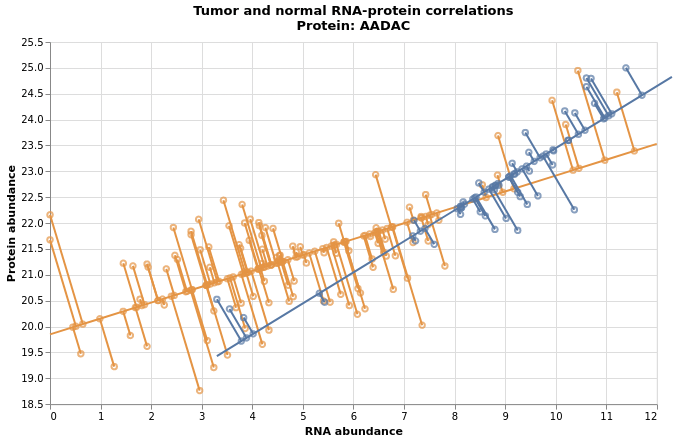
\includegraphics[width=0.5\textwidth]{deltacorr}
    \caption{RNA to protein correlation plot for a single protein. Orange is tumor, blue is normal; orthogonal residuals are shown. Delta correlation is the difference between the tumor correlation coefficient and the normal correlation coefficient.}
    \label{fig:deltacorr}
\end{figure}

After calculating these tumor-normal residual differences for the overall most important proteins in each patient, and the above or below regression line data for each protein in each patient, we calculated correlation between tumor and normal residuals for each patient in across all proteins. This used the Spearman method again, and provided with a single new feature for each patient, based on the delta correlation data.

\begin{figure}[H]
    \centering
    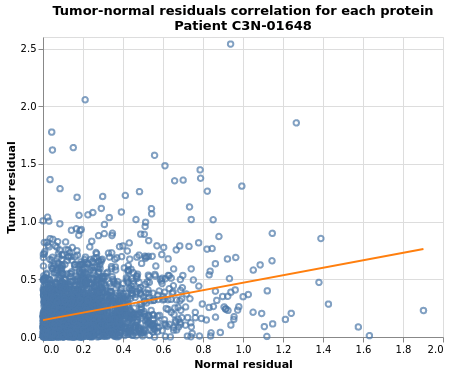
\includegraphics[width=0.5\textwidth]{tn_resid_corr}
    \caption{Normal residual to tumor residual correlation plot for a single patient.}
    \label{fig:tn_resid_corr}
\end{figure}

\begin{figure}[H]
    \centering
    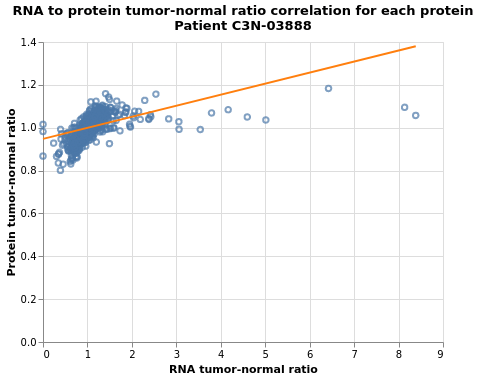
\includegraphics[width=0.5\textwidth]{tn_ratio_corr}
    \caption{RNA tumor-normal ratio to protein tumor-normal ratio correlation plot for a single patient.}
    \label{fig:tn_ratio_corr}
\end{figure}

Our final feature was not derived from the delta correlations. Instead, for each protein in each patient, we calculated the ratio of tumor RNA abundance to normal RNA abundance and the ratio of tumor protein abundance to normal protein abundance, then found the correlation for each patient between this RNA tumor-normal ratio and this protein tumor-normal ratio across all proteins. The goal was to generate a feature for each patient that reflected differences between RNA and protein data, but, unlike the delta correlation-derived data, did not depend on data across multiple patients, and thus could be calculated for a single new patient without needing to find how that data fit in with data from other patients.

\subsubsection{Targets}

Clinical data was obtained in the same manner as proteomics and transcriptomics data. For targets, we selected six categorical features that had lower numbers of missing values and had potential to be predictable based on our input features. The targets chose were survival status, recurrence status, and treatment success status of the patient at last follow-up, as well as histologic grade and type, and tumor stage.

\subsection{Data cleaning}

For boolean input features (the above or below regression line features), missing values were filled randomly with true and false values in such a way that the imputed data would have the same proportion of true to false values as the original data. Missing values in numerical features were filled with the mean of the feature, and all numerical features were normalized using the formula $(x - min(x)) / (max(x) - min(x))$.

\subsection{Scoring}

We used three scoring metrics: accuracy, precision, and recall. Accuracy is simply the proportion of samples that were correctly scored. Precision and recall are based on the confusion matrix for the scoring results. For a single class, precision is calculated as $\frac{TP}{TP + FP}$, where $TP$ is the true positive rate and $FP$ is the false positive rate. It tells us what proportion of samples assigned the given class were actually in that class. Recall for a single class is calculated as $\frac{TP}{TP + FN}$, where $TP$ is the true positive rate and $FN$ is the false negative rate. This tells us what proportion of all members of the given class were successfully detected as members of that class. Thus, if we have high precision we know that anything assigned the given class is probably actually in that class; if we have high recall, we know that anything that is actually in the given class was probably assigned to that class.

In our data, some targets have more than two output classes. In these cases, precision and recall are calculated separately for each output class, and then averaged across all output classes.

\section{Results}

\subsection{Baseline accuracy}

To establish a baseline accuracy for the targets, we trained the SciKit Learn multi-layer perceptron (MLP) using the default hyperparameters, except reducing the hidden layers to one layer of 16 nodes, supposing that this simple model would give us a good idea of the complexity of the problem. The cancer type input feature, as well as all targets, were one-hot encoded. Testing with 10-fold cross-validation yielded these baseline results for each target:

\medskip

\begin{table}[H]
\begin{center}
\begin{tabular}{ *{4}{l} }
    \multicolumn{1}{p{1.5cm}}{\raggedright Target} &  
    \multicolumn{1}{p{1.5cm}}{\raggedright Accuracy} &  
    \multicolumn{1}{p{1.5cm}}{\raggedright Precision} &  
    \multicolumn{1}{p{1.5cm}}{\raggedright Recall} \\ \hline
histologic\_grade       &         0.3309 &          0.3371 &       0.3434 \\
histologic\_type        &         0.1949 &          0.1949 &       0.1949 \\
recurrence\_status      &         0.7702 &          0.7733 &       0.7764 \\
success\_last\_follow-up &         0.2570 &          0.2585 &       0.2600 \\
survival\_status        &         0.8067 &          0.8113 &       0.8159 \\
tumor\_stage            &         0.3578 &          0.3761 &       0.3945 \\
\end{tabular}
\caption{Baseline scores for each target.}
\end{center}
\end{table}

\subsection{Multi-layer perceptron}

After establishing the baseline accuracy using an MLP, we initially tried to optimize all hyperparameters at once using the SciKit Learn randomized cross-validation search. This method draws random combinations of hyperparameters from user-provided distributions and tests them, returning the best combinations it finds. This did lead to improvements in all metrics for the "histologic\_grade" and "success\_last\_follow-up" targets, and a marginal improvement in the recall for "recurrence\_status", as shown below:

\medskip

\begin{table}[H]
\begin{center}
\begin{tabular}{ *{4}{l} }
    \multicolumn{1}{p{1.5cm}}{\raggedright Target} &  
    \multicolumn{1}{p{1.5cm}}{\raggedright Accuracy} &  
    \multicolumn{1}{p{1.5cm}}{\raggedright Precision} &  
    \multicolumn{1}{p{1.5cm}}{\raggedright Recall} \\ \hline
histologic\_grade       &              \textbf{0.3669} &               \textbf{0.3822} &            \textbf{0.4012} \\
histologic\_type        &              0.1411 &               0.1441 &            0.1599 \\
recurrence\_status      &              0.7653 &               0.7711 &            \textbf{0.7769} \\
success\_last\_follow-up &              \textbf{0.3085} &               \textbf{0.3208} &            \textbf{0.3473} \\
survival\_status        &              0.7990 &               0.8005 &            0.8021 \\
tumor\_stage            &              0.2059 &               0.2170 &            0.2282 \\
\end{tabular}
\caption{MLP scores for each target after initial random hyperparameter search.}
\end{center}
\end{table}

However, for the rest of the targets this random search actually led to decreased scores. We believe this is because it takes too many iterations to happen upon good parameter combinations if all parameters were being randomly selected at once. So, we instead decided to only use the random search to optimize one hyperparameter at a time, holding all others constant. Using this method, we obtained the following results for each target. This led to significant score improvements for "histologic\_grade", "histologic\_type", "success\_last\_follow-up", and "tumor\_stage".

\medskip
\begin{table}[H]
\begin{center}
\begin{tabular}{ *{4}{l} }
    \multicolumn{1}{p{1.5cm}}{\raggedright Target} &  
    \multicolumn{1}{p{1.5cm}}{\raggedright Accuracy} &  
    \multicolumn{1}{p{1.5cm}}{\raggedright Precision} &  
    \multicolumn{1}{p{1.5cm}}{\raggedright Recall} \\ \hline
histologic\_grade       &       \textbf{0.521496} &        \textbf{0.521496} &     \textbf{0.521496} \\
histologic\_type        &       \textbf{0.593371} &        \textbf{0.600994} &     \textbf{0.608617} \\
recurrence\_status      &         0.7702 &          0.7733 &       0.7764 \\
success\_last\_follow-up &       \textbf{0.517803} &        \textbf{0.517803} &     \textbf{0.517803} \\
survival\_status        &         0.8067 &          0.8113 &       0.8159 \\
tumor\_stage            &       \textbf{0.366288} &        \textbf{0.409233} &     \textbf{0.452178} \\
\end{tabular}
\caption{MLP scores for each target after targeted hyperparameter searching.}
\end{center}
\end{table}

\subsection{k-nearest neighbors}

The first parameter that was optimized was k. We found that accuracy ceased to improve once k \textgreater  20. 
As with MLP, we tested a combination of hyperparameters. 
Due to the speed of KNN we were able to test a wide range of parameters. We were able to test every possible input for weights (the weight function used in prediction), algorithm (the algorithm used to compute the nearest neighbors), and p (the parameter for the Minkowski metric). 
n\_neighbors and leaf\_size tested a range of numbers, 10-100 and 2-50 respectively.
The optimal scores for each target are reported in the table below.

\medskip
\begin{table}[H]
\begin{center}
\begin{tabular}{ *{4}{l} }
    \multicolumn{1}{p{1.5cm}}{\raggedright Target} &  
    \multicolumn{1}{p{1.5cm}}{\raggedright Accuracy} &  
    \multicolumn{1}{p{1.5cm}}{\raggedright Precision} &  
    \multicolumn{1}{p{1.5cm}}{\raggedright Recall} \\ \hline
histologic\_grade         &              \textbf{0.3882} &               \textbf{0.3882} &            \textbf{0.3882} \\
histologic\_type          &              0.0164 &               0.0164 &            0.0164 \\
recurrence\_status        &              \textbf{0.8126} &               \textbf{0.8126} &            \textbf{0.8126} \\
success\_last\_follow-up  &              \textbf{0.3066} &               \textbf{0.3066} &            \textbf{0.3066} \\
survival\_status          &              \textbf{0.8250} &               \textbf{0.8250} &            \textbf{0.8250} \\
tumor\_stage              &              0.1043 &               0.1043 &            0.1043 \\
\end{tabular}
\caption{KNN scores for each target.}
\end{center}
\end{table}

\subsection{Naïve Bayes}
SciKit Learn does not currently have a Naïve Bayes classifier that takes both continuous data and nominal data. We separated the continuous data from the nominal and then ran Sci-Kit's GaussianNB classifier on the continuous data and Sci-Kit's MultinomialNB on the nominal data. Again, we used 10-fold cross validation and took the average accuracy, precision, and recall scores. The MultinomialNB classifier scored similarly to the MLP, however the GaussianNB classifier performed poorly across all labels with accuracies ranging between 10 and 50 percent.

\begin{table}[H]
  \begin{center}
  \begin{tabular}{ *{4}{l} }
      \multicolumn{1}{p{1.5cm}}{\raggedright Target} &  
      \multicolumn{1}{p{1.5cm}}{\raggedright Accuracy} &  
      \multicolumn{1}{p{1.5cm}}{\raggedright Precision} &  
      \multicolumn{1}{p{1.5cm}}{\raggedright Recall} \\ \hline
histologic\_grade         &       \textbf{0.3499} &        \textbf{0.3499} &     \textbf{0.3499} \\
histologic\_type          &       \textbf{0.4776} &        \textbf{0.4776} &     \textbf{0.4776} \\
recurrence\_status        &       0.2570 &        0.2570 &     0.2570 \\
success\_last\_follow-up  &       0.1435 &        0.1435 &     0.1435 \\
survival\_status          &       0.4482 &        0.4482 &     0.4482 \\
tumor\_stage              &       \textbf{0.3997} &        \textbf{0.3997} &     \textbf{0.3997} \\
\end{tabular}
\caption{Scores for GaussianNB on continuous data.}
\end{center}
\end{table}

\begin{table}[H]
  \begin{center}
  \begin{tabular}{ *{4}{l} }
      \multicolumn{1}{p{1.5cm}}{\raggedright Target} &  
      \multicolumn{1}{p{1.5cm}}{\raggedright Accuracy} &  
      \multicolumn{1}{p{1.5cm}}{\raggedright Precision} &  
      \multicolumn{1}{p{1.5cm}}{\raggedright Recall} \\ \hline
histologic\_grade        &       \textbf{0.4512} &        \textbf{0.4512} &     \textbf{0.4512} \\
histologic\_type         &       \textbf{0.5581} &        \textbf{0.5581} &     \textbf{0.5581} \\
recurrence\_status       &       \textbf{0.8098} &        \textbf{0.8098} &     \textbf{0.8098} \\
success\_last\_follow-up &       \textbf{0.5121} &        \textbf{0.5121} &     \textbf{0.5121} \\
survival\_status         &       \textbf{0.8253} &        \textbf{0.8253} &     \textbf{0.8253} \\
tumor\_stage             &       \textbf{0.5271} &        \textbf{0.5271} &     \textbf{0.5271} \\
\end{tabular}
\caption{Scores for MultinomialNB on nominal data.}
\end{center}
\end{table}

\section{Discussion}

Our analysis yielded mixed results. For the recurrence and survival targets, our dataset is not large enough to successfully learn this problem. The best accuracies we achieved for those two features were both around 80\%; however, both features have about 80\% of patients in one class and 20\% in the other, so the models achieved this accuracy simply by guessing the majority class every time, and not really paying attention to any differences between samples. If we obtained a larger dataset, that would enable our models to learn more deeply about these features.

Our model did perform slightly better on the other 4 targets. However, the best accuracies were still not hugely better than the proportion of samples that were in the majority class for the target, indicating again that our models were likely over-reliant on assuming the majority class from the training data. Again, a larger dataset would be the best way to address this issue.

Additionally, the performance differences of the two different Naïve Bayes classifiers suggests that the nominal features are more indicative of outcomes than the continuous data.

\section{Conclusion and future directions}

Our analysis successfully improved our prediction accuracies compared to the baseline scores. However, our best accuracies on each target were consistently similar to the proportion of samples in the majority class for that target, indicating an over-reliance in the models of just assuming the majority class found in the training data. This limitation is primarily due to the small number of samples we have for such a complex dataset. Quantitative proteomic and transcriptomic data are notorious for containing large amounts of noise, and it appears that in this situation, the noise prevented successful learning from the small number of samples we have.

Future directions include obtaining more training data. Although it would be expensive to augment as comprehensive of a dataset as CPTAC's, that is an eventual goal for all proteogenomic cancer research. The CPTAC dataset is certainly the best we have so far, but there is much more that needs to be done in the future as sample analysis capabilities improve. However, before that time comes, additional work could be done in our current workflow to improve the features we're working with. For example, our simple metric of including the residual differences from the proteins with the top 25 largest delta correlations leaves out huge amounts of data. A more nuanced selection or pooling calculation would likely improve the utility of the feature. Similar possibilities exist for the other feature calculations we performed.

%% The file named.bst is a bibliography style file for BibTeX 0.99c
\bibliographystyle{named}
\bibliography{dcml}

\end{document}

